\chapter{Zastosowania praktyczne}

\section{Wprowadzenie}

Rozdział ten skupia się na potencjalnych zastosowaniach praktycznych dla problemu WCRDF oraz poszukiwania $\gamma^{\text{wc}}_R(G)$. Patrząc na genezę historyczną problemu, warto poszukać zastosowań w życiu codziennym, w celu maksymalizacji ochrony przy niskim jej koszcie\cite{theoryWCRDF}.\\
Literatura proponuje parę zastosowań. Jednym z nich jest próba optymalnego rozmieszczenia pojazdów służb ratunkowych. Utrzymanie i kupno takiego pojazdu jest kosztowne, ale jednocześnie cała sieć budynków służb ratunkowych powinna mieć szybki dostęp do takiego pojazdu, aby móc dotrzeć do potrzebujących. Pojazdy można rozmieścić na wzór legionów rzymskich, w budynkach służb ratunkowych powinien znajdować się pojazd, bądź być możliwość wypożyczenia go z sąsiedniej (najbliższej) lokalizacji służb ratunkowych\cite{improvedILP}.\\
W rozdziale przeprowadzono analizę potencjalnych zastosowań:
\begin{itemize}
    \item rozmieszczenie zabezpieczeń sieci energetycznych,
    \item rozmieszczenie agentów wykrywających oszustwa w internetowej sieci
    społecznościowej.
\end{itemize}
Warto zaznaczyć, że oba zastosowania są potencjalne i teoretyczne, nie została przeprowadzona analiza dotycząca faktyczngo działania wykorzystywanych systemów.\\
Do analizy zostały wykorzystane prawdziwe lub uproszczone grafy występujące w rzeczywistości. Następnie grafy te poddano działaniom wybranych algorytmów, tam gdzie było to możliwe. Dodatkowo dokonano analizy jakościowej i czasowej tych algorytmów, w kontekście analizowanego zastosowania.

\section{Rozmieszczenie zabezpieczeń sieci energetycznych}

Inspiracją tego zastosowania był blackout na półwyspie Iberyjskim pod koniec kwietnia 2025 roku\cite{BLACKOUT}, w którym w wyniku awarii początkowo jednej podstacji, doszło do wyłączenia prądu w kilku krajach. \\
Dlatego propozycją zapobiegania takim problemom może być próba rozmieszczenia systemów alternatywnych lub zabezpieczających takich, które mogą ochronić albo przejąć obciążenie wadliwej stacji energetycznej, aby zapobiec większej awarii. Dominowanie rzymskie słabo spójne będzie miało tutaj zastosowanie ze względu na chęć utrzymania komunikacji między stacjami energetycznymi. Naturalnie, takie systemy wiążą się z niemałymi kosztami, a więc warto, aby było ich jak najmniej. Zatem zastosowanie algorytmów rozwiązujących problem minimalnej WCRDF wydaje się odpowiednie, przynajmniej w ujęciu teoretycznym.\\
W tym przypadku jako graf można przyjąć stacje energetyczne i transformatory, natomiast jako krawędzie można przyjąć sieci energetyczne, czyli połączenia między stacjami i transforamtorami.\\
W celu próby realizacji tego pomysłu zbudowano graf połączeń sieci i stacji energetycznych najwyższych napięć w Polsce\cite{POLAND}. W praktyce sieć jest bardziej rozbudowana, jednakże tutaj skupiono się na najwyższym napięciu 400kV. Jej graf przedstawiono na tle mapy Polski. Z powierzchownej analizy tego grafu można zauważyć, że jest to graf bardzo rzadki, posiada wiele wierzchołków o niskim stopniu. Cechuje się brakiem hubów, nie ma wierzchołków o dużym stopniu.
//TU DODAĆ ZDJECIE GRAFU POLSKI I PODAĆ LICZBE WIERZCHOŁKÓW I KRAWĘDZI.
Dla grafów bardzo rzadkich, na podstawie analizy z poprzedniego rozdziału można wysnuć hipotezę, że algorytmy programowania liniowego z racji niewielkiej liczby krawędzi będą dawały optymalne wyniki w rozsądnym czasie dla tej skali problemu. Algorytm zachłanny powinien prezentować dobry stosunek jakości do czasu działania. Jeśli chodzi o algorytm Approx, z racji rzadkiego grafu, może on prezentować gorszą jakość rozwiązania.\\

Poniższe grafiki przedstawiają wyniki działania algorytmów ILP2, Greedy oraz Approx. Standardowo, żółte wierzchołki to 0, niebieskie to 1, a czerwone to 2.

\begin{figure}[htbp]
    \centering
    \begin{subcaptionbox}{ILP2\label{fig:img}}[0.48\linewidth]
        {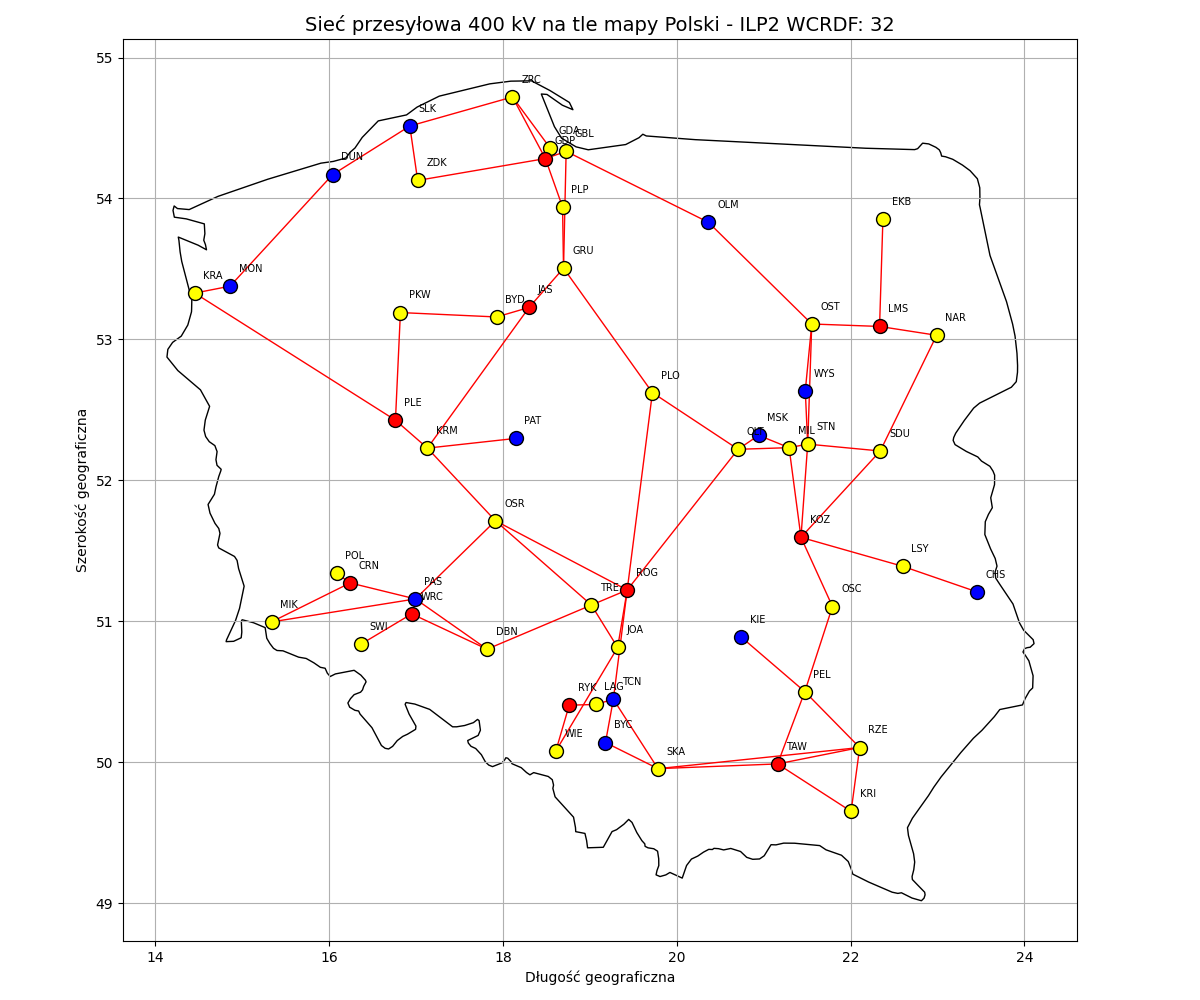
\includegraphics[width=\linewidth]{assets/Poland/img.png}}
    \end{subcaptionbox}
    \hfill
    \begin{subcaptionbox}{Greedy\label{fig:img2}}[0.48\linewidth]
        {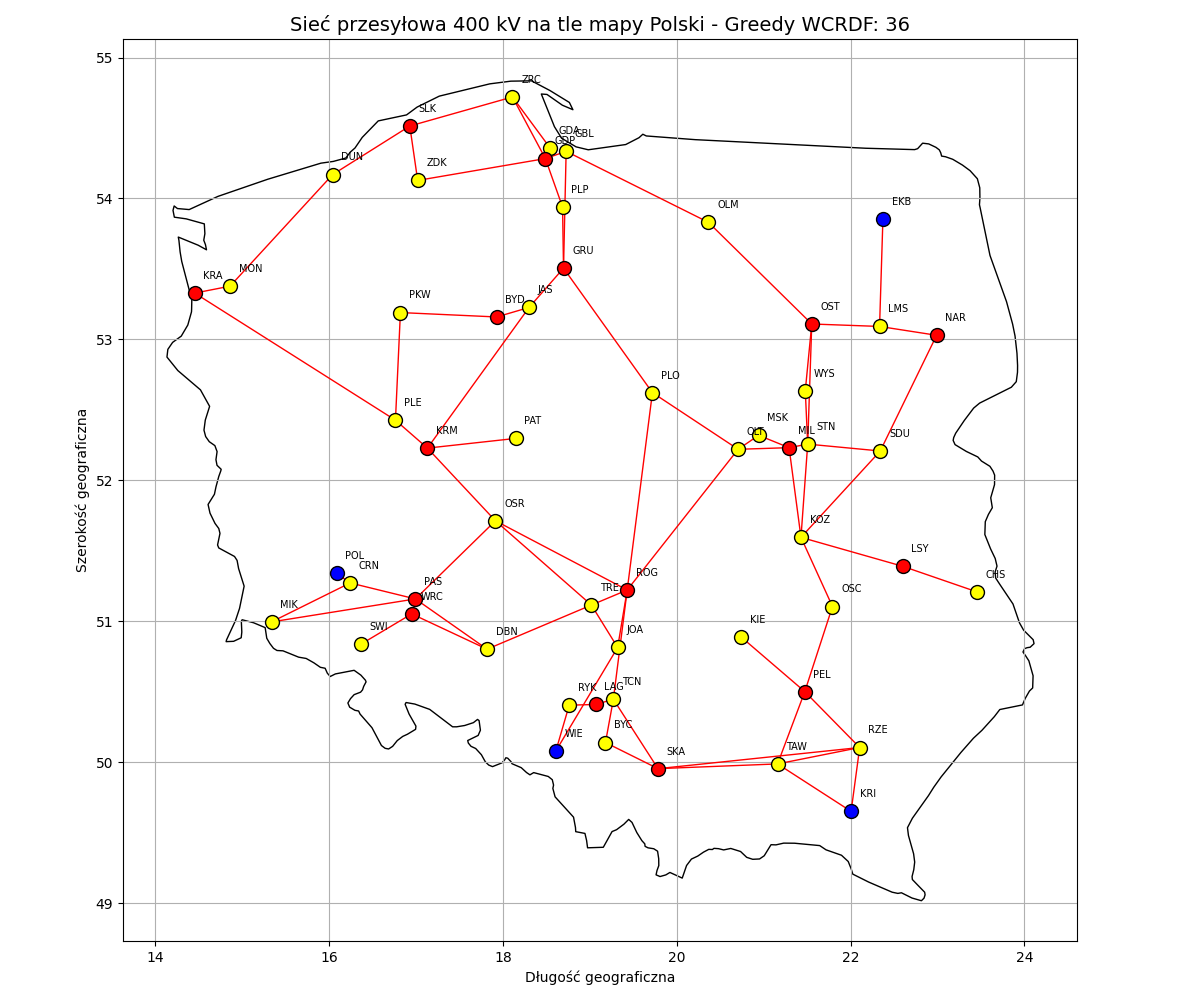
\includegraphics[width=\linewidth]{assets/Poland/img_2.png}}
    \end{subcaptionbox}
    \hfill
    \begin{subcaptionbox}{Approx\label{fig:img1}}[0.48\linewidth]
        {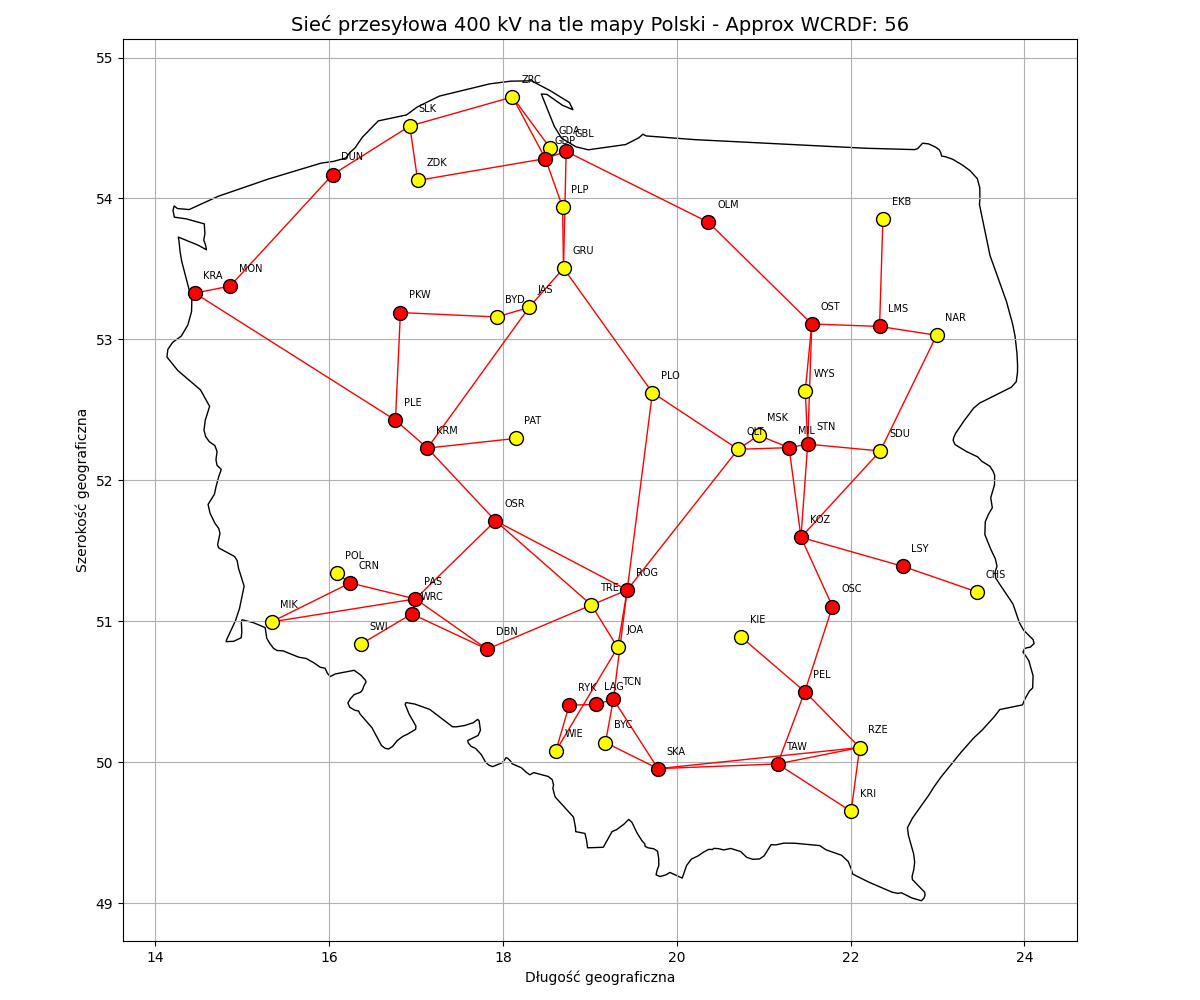
\includegraphics[width=\linewidth]{assets/Poland/img_1.png}}
    \end{subcaptionbox}
    \caption{Efekt działania algorytmów ILP, Greedy i Approx dla problemu rozmieszczenia zabezpieczeń sieci energetycznych.}
    \label{fig:poland}
\end{figure}

\begin{table}[H]
    \centering
    \begin{tabular}{|c|c|c|}
        \hline
    Algorytm & $\gamma^{\text{wc}}_R(G)$ & Czas działania [s] \\     \hline
    ILP2 & 32 & 2,7014378 \\ \hline
    Greedy & 36 & 0,0003222 \\ \hline
Approx & 56 & 647,6564676 \\ \hline
\end{tabular}
\caption{Wynik działania wybranych algorytmów dla problemu rozmieszczenia zabezpieczeń sieci energetycznych.}
\end{table}

Algorytmowi ILP2 udało odnaleźć optymalne rozwiązanie w ciągu dwóch sekund, co jest bardzo dobrym wynikiem. Nieznacznie gorszy wynik prezentuje algorytm zachłanny. Natomiast zgodnie z przewidywaniami, algorytm Approx osiągnął znacznie gorszy wynik od pozostałych, ze względu na to, że szuka on zbioru dominującego spójnego, co w przypadku grafu bardzo rzadkiego mocno zawyża wyniki. Charakteryzuje się też znacznie dłuższym czasem działania od pozostałych.\\

To rozważanie pokazuje, że nawet dla nieco większych grafów rzadkich, obserwowanych w rzeczywistym życiu, można dokładnie rozwiązać problem $\gamma^{\text{wc}}_R(G)$, dzięki algorytmom programowania liniowego i nie ma konieczności stosowania algorytmów przybliżonych. Jednakże, warto podkreślić tutaj potencjał algorytmu zachłannego, który osiągnął nieznacznie gorszy wynik, a jest bez wątpienia najbardziej skalowalnym algorytmem ze wszystkich prezentowanych.

\section{Rozmieszczenie agentów wykrywających oszustwa w internetowej sieci społecznościowej}

\begin{figure}[htbp]
    \centering
    \begin{subcaptionbox}{ILP, $\gamma^{\text{wc}}_R(G)$: 7\label{fig:ilp}}[0.48\linewidth]
        {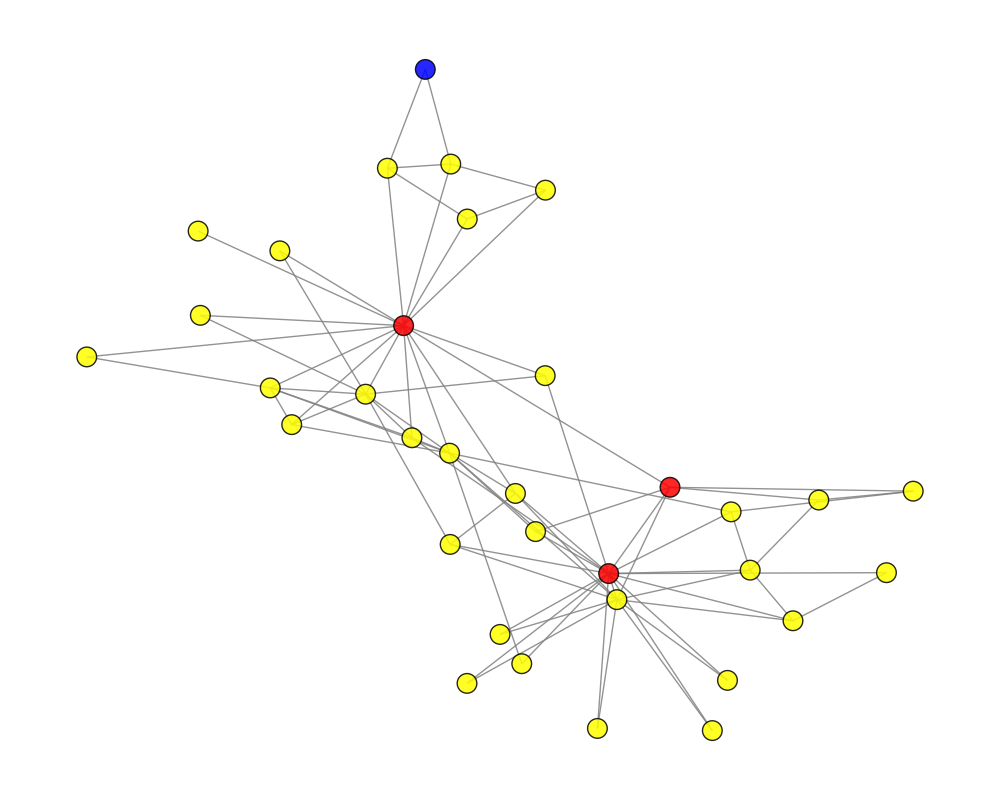
\includegraphics[width=\linewidth]{assets/Facebook/ilp.png}}
    \end{subcaptionbox}
    \hfill
    \begin{subcaptionbox}{ILP2,  $\gamma^{\text{wc}}_R(G)$: 7\label{fig:ilp2}}[0.48\linewidth]
        {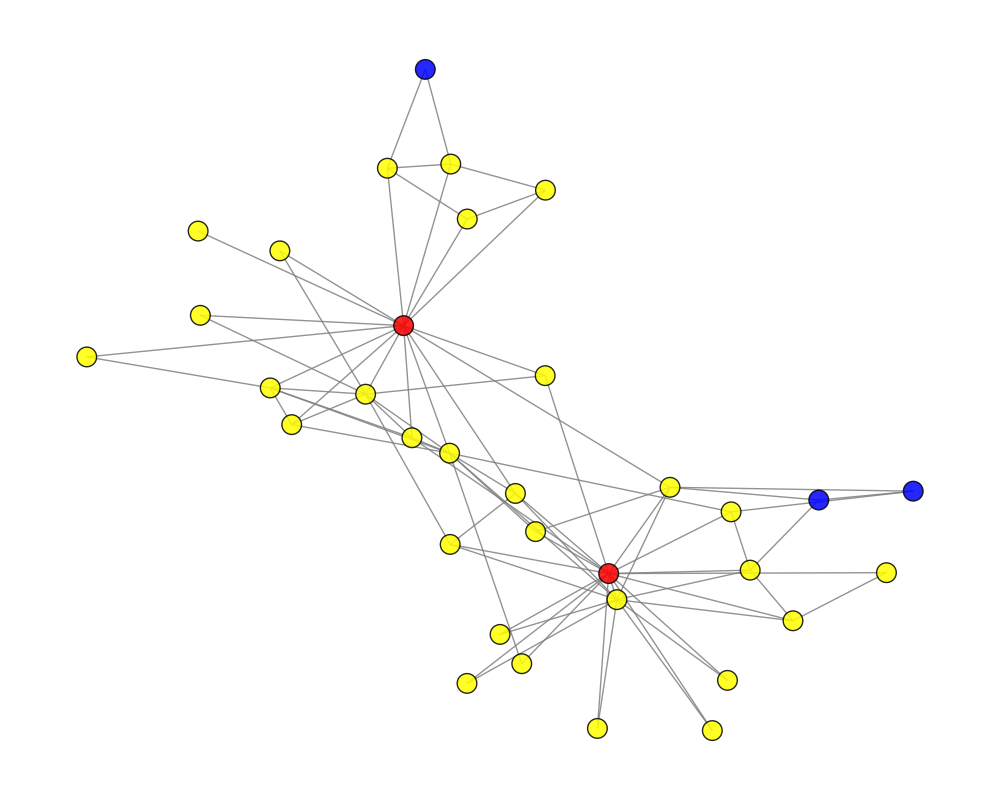
\includegraphics[width=\linewidth]{assets/Facebook/ilp2.png}}
    \end{subcaptionbox}
    \hfill
    \begin{subcaptionbox}{Greedy  $\gamma^{\text{wc}}_R(G)$: 7\label{fig:greedy}}[0.48\linewidth]
        {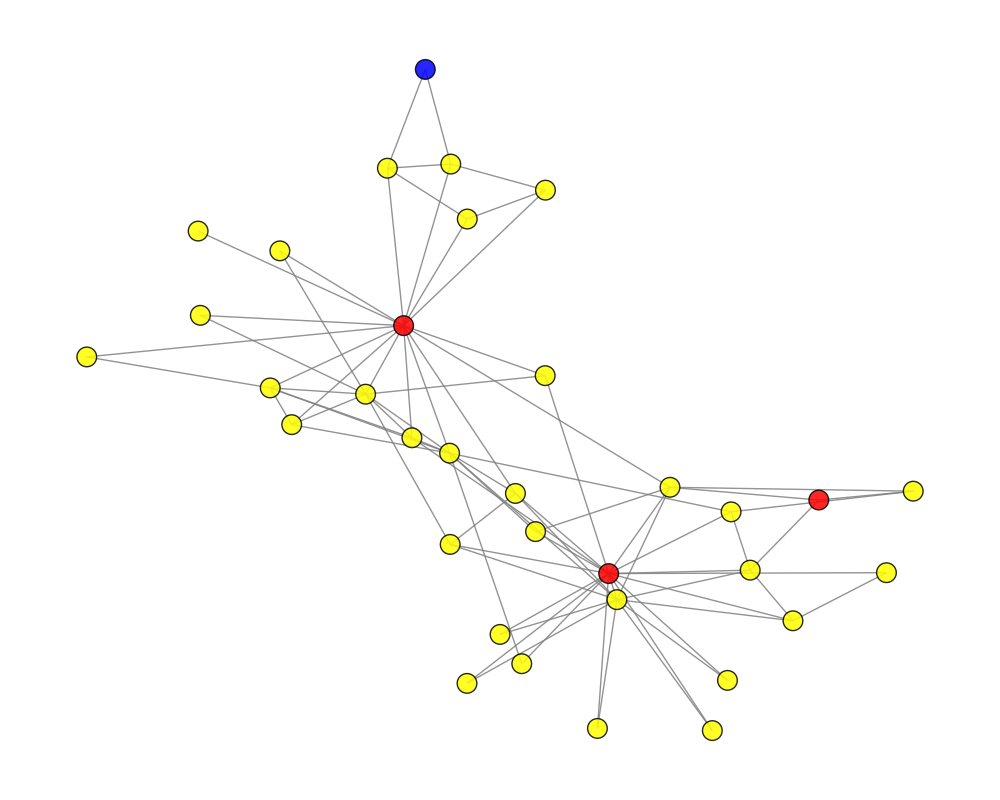
\includegraphics[width=\linewidth]{assets/Facebook/greedy.png}}
    \end{subcaptionbox}
    \hfill
    \begin{subcaptionbox}{Approx  $\gamma^{\text{wc}}_R(G)$: 8\label{fig:approx}}[0.48\linewidth]
        {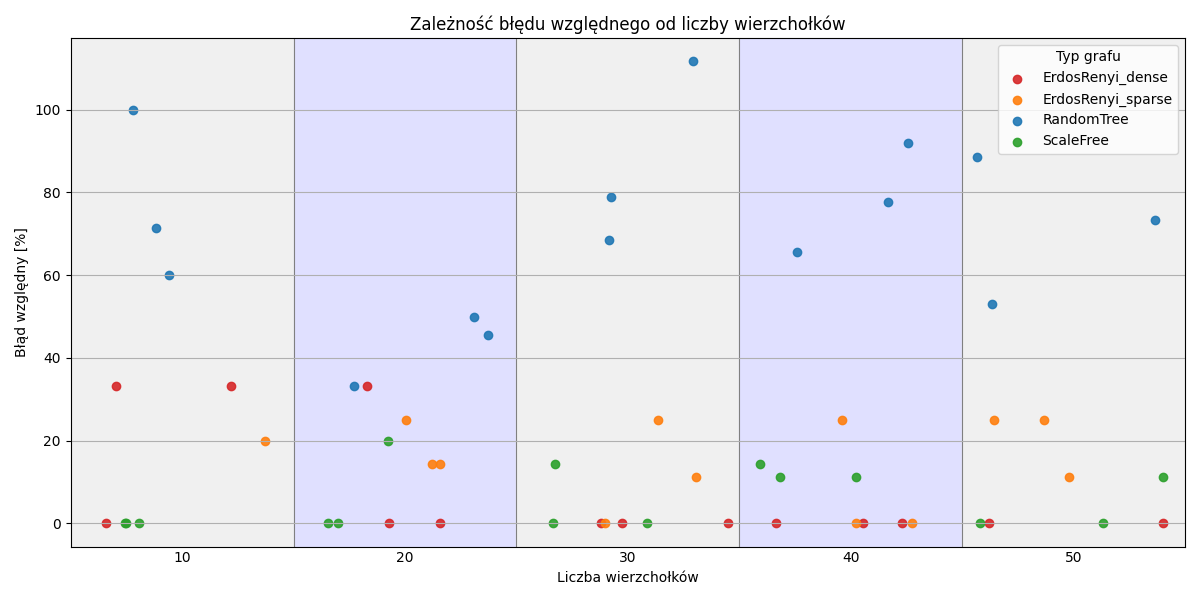
\includegraphics[width=\linewidth]{assets/Facebook/approx.png}}
    \end{subcaptionbox}
    \hfill
    \begin{subcaptionbox}{AntColony  $\gamma^{\text{wc}}_R(G)$: 21\label{fig:ant}}[0.48\linewidth]
        {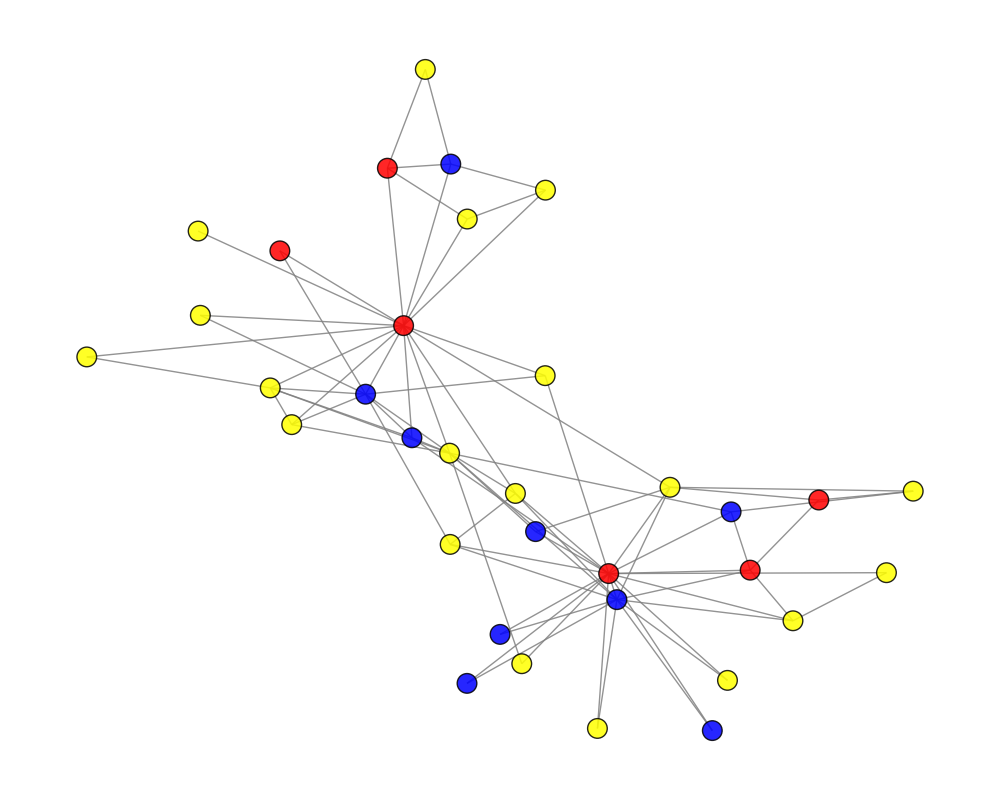
\includegraphics[width=\linewidth]{assets/Facebook/ant.png}}
    \end{subcaptionbox}

    \caption{Efekt działania algorytmów ILP, Greedy i Approx dla problemu rozmieszczenia agentów w małej, rzeczywistej sieci społecznościowej.}
    \label{fig:karate}
\end{figure}

\begin{table}[H]
    \centering
    \begin{tabular}{|c|c|c|}
        \hline
    Algorytm & $\gamma^{\text{wc}}_R(G)$ & Czas działania [s] \\     \hline
    ILP2 & 7 & 0,0865662 \\ \hline
    ILP & 7 & 0,0624058 \\ \hline
    Greedy & 7 & 0,0001245 \\ \hline
    Approx & 8 & 0,1533187 \\ \hline 
    AntColony & 21 & 5,1319121 \\ \hline
\end{tabular}
\caption{Wynik działania wybranych algorytmów dla problemu rozmieszczenia agentów w małej sieci społecznościowej.}
\end{table}

\begin{figure}[H]
    \centering
    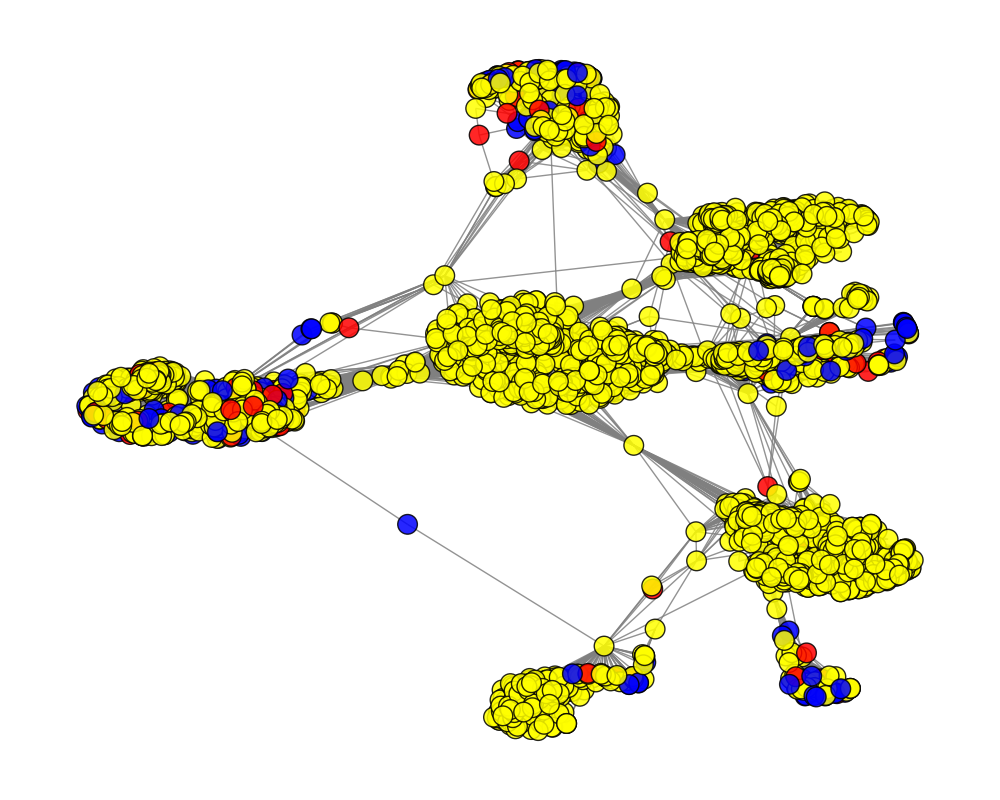
\includegraphics[width=0.75\textwidth]{assets/Facebook/facebookgreedy.png}
    \caption{Efekt działania algorytmu zachłannego dla problemu rozmieszczenia agentów w dużej, rzeczywistej sieci społecznościowej. $\gamma^{\text{wc}}_R(G)$: 411, czas działania 2,9348995 s.}
    \label{fig:fbgreedy}
\end{figure}